\begin{kasten}
  \section*{ \hspace{0.1cm} {\color{red} \underline{DEFINING THE MODEL}}}
  \large{
    \begin{minipage}{4cm}
      POM2 implements four of the five scales identified by Boehm and Turner that distinguish agile from traditional
      plan-based projects: 
      \begin{smallitem}
      \item Criticality
      \item Dynamism
      \item Culture
      \item Size
      \end{smallitem}
      \vspace{3 mm}
      Boehm and Turner measure criticality in terms of losses due
    \end{minipage}
    \begin{minipage}{9cm}
      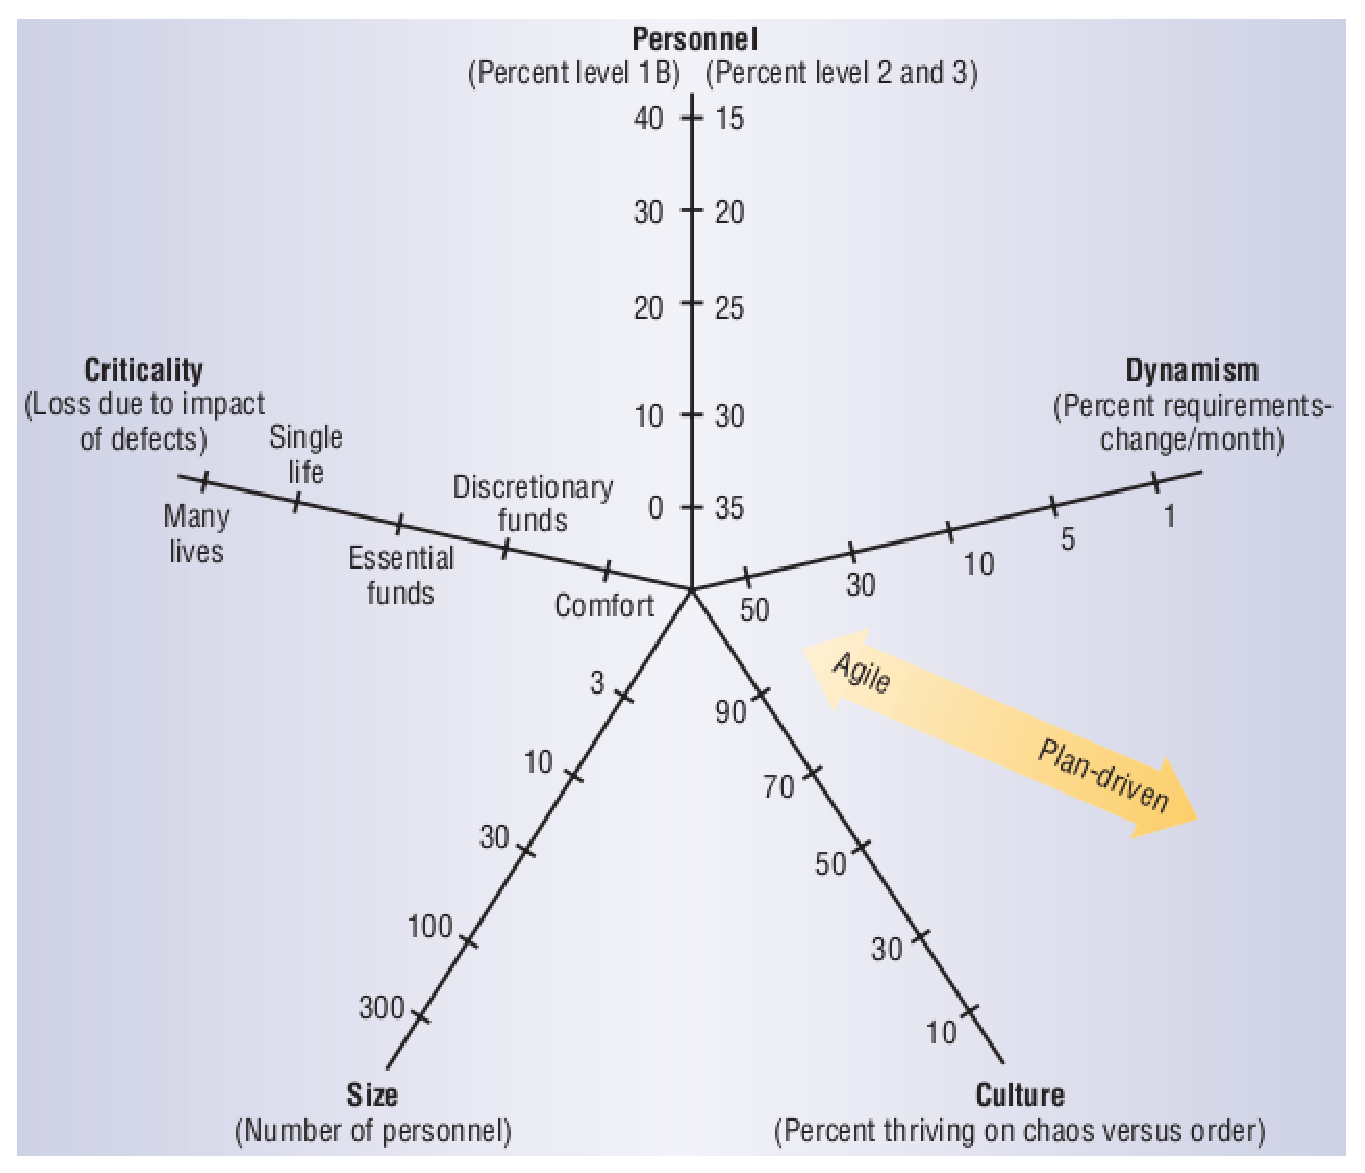
\includegraphics[width=9cm]{star.eps}
    \end{minipage}
 to defects, it ranges from ``none'' (best for agile development) 
      to     ``loss of many lives'' (must be carefully planned, suited for plan-based approach).  In POM2 X\% of the requirements
    are affected by criticality, where \begin{math} X = 2...10 \end{math}. Each requirement in a team's tree is adjusted 
    using the equation: \begin{equation} cost' = cost * X^{criticality} \end{equation}

    \vspace{3 mm}
    Dynamism measures how frequently new requirements are created and their values change.  Boehm and Turner measure dynamism 
    in terms of percent of requirements changed each month, and has the range 50\% (best for agile) to 1 (best for plan-based).
    In POM2 we implement this as follows:
    \begin{smallitem}
    \item Initially only 30\% to 70\% of the requirements in the project tree are ``visible''.
    \item After each iteration we make visible \begin{math} new = Poisson(\lambda) \end{math} more requirements.
    \item Dynamism also affects the value of already visible requirements.  The value is adjusted using the equation:
      \begin{equation} value' += maxValue * N(0,\sigma) \end{equation}
    \item After setting \begin{math}\sigma\end{math} , we set \begin{math}\lambda\end{math} to 10\% of \begin{math}\sigma\end{math}.
    \end{smallitem}

    Culture, according to Boehm and Turner is measured in terms of the percent of the staff thriving on chaos, ranging from
    10\% (best for plan-based) to 90\% (best for agile).  In POM2 culture is handled through an accepted value associated with 
    each requirement.  The calculation for the accepted value is: \begin{equation} value + (value N(0,\sigma)*culture) \end{equation}
    
    \vspace{3 mm}
    Size is measured in terms of the number of personnel and has a range of 3 (best for agile), 10, 30, 100, 300 (best for plan-based).
    In POM2 this size is picked randomly and dictates the number of requirements in the project:
    \begin{equation} \mathtt{\mbox{\textit{number of requirements}}} = size * 2.5 \end{equation}
    
    \vspace{3 mm}
    The one scale we did not implement was personnel.  Boehm and Turner describe personnel using the Cockburn mixtures model of Alpha, Beta and Gamma programmers:
    \begin{smallitem}
    \item Alpha: Most productive/flexible programmers.
    \item Beta: Able to perform discretionary method steps.
    \item Gamma: Unable/unwilling to follow shared methods.
    \end{smallitem}
    By the conventions of the Boehm and Turner personnel scale, lower personnel values indicate more alpha programmers.
    Combining the COCOMO effort multipliers and the Cockburn mixtures model, the net effect is nearly zero.  For that reason,
    POM2 ignores personnel and will address it in future work.
    \vspace{1em}
  }
\end{kasten}
